            %\documentclass[a4,semhelv,landscape]{seminar}
\documentclass[landscape]{slides}
%\documentclass[pdf, default, slideBW, nocolorBG]{prosper}
\usepackage[left=1.0cm,top=0.2cm,right=1.0cm,nohead,nofoot]{geometry}
%\def\everyslide{\sffamily}
%\usepackage{fullpage}
\usepackage{graphicx}
\usepackage{setspace}
\usepackage{xcolor}
\usepackage{color}
\usepackage{fancyvrb}
\usepackage{verbatim}
\usepackage{nopageno}
%\usepackage{times}
% define some nice colors
\definecolor{myred}{rgb}{0.6,0,0}
\definecolor{myblue}{rgb}{0,0.2,0.4}
\def\imagetop#1{\vtop{\null\hbox{#1}}}
%\color{myblue}

%\DefineVerbatimEnvironment{sreoutput}{Verbatim}{fontsize=\scriptsize,xleftmargin=10.0\parindent}%
\DefineVerbatimEnvironment{sreoutput}{Verbatim}{fontsize=\small,xleftmargin=10.0\parindent}%
\DefineVerbatimEnvironment{sreoutput2}{Verbatim}{fontsize=\tiny,xleftmargin=10.0\parindent}%
%\input{macros}

\begin{document}
%%%%%%%%%%%%%%%%%%%%%%%%%%%%%%%%%%%%%%%%%%%%%%%%%%%%%%%%%%%%%%%%%%%%%%%%%%
\begin{slide}

\center{\large{\textbf{Updating SSU-ALIGN and \\ searching for Group I Introns}}}
\normalsize

11.03.14

\medskip

%\includegraphics[width=3in]{figs/ssualign-logo}

\small

%\begin{tabular}{c}
%Janelia Farm Research Campus \\
%Howard Hughes Medical Institute \\ 
%\\
%Deparment of Genetics \\
%Washington University in St. Louis \\
%\\
%%& & Washington University in St. Louis \\
%\end{tabular}%
%
%\includegraphics[width=2.25in]{figs/janelia}
%\hspace{2in}
%\includegraphics[width=1.75in]{figs/washu}

%\end{center}
\end{slide}
%%%%%%%%%%%%%%%%%%%%%%%%%%%%%%%%%%%%%%%%%%%%%%%%%%%%%%%%%%%%%%%%%%%%%%%%%%
\begin{slide}
\begin{center}

\textbf{SSU rRNA is especially abundant in sequence datasets}
\end{center}
\medskip
\begin{minipage}{7in}
\small
\begin{itemize}
\item mid 1980s - Norman Pace develops methodology for determination
      of SSU sequences without cultivation
\item many different environments have been surveyed
\item known biodiversity has been greatly expanded:

\begin{itemize}
\item
  recognized bacterial phyla: \\
  11 in 1987, 36 in 1998, 52 in 2003, 67 in 2006...
\end{itemize}

\item SSU databases contain millions of sequences:
\begin{center}
\begin{tabular}{lrr}
  name & \# seqs & \# citations \\ \hline
  Silva & 3.2M & 1125 \\ 
  RDP   & 2.6M & 1170 \\
  Greengenes & 1.0M & 1012 \\
\end{tabular}
\end{center}
\end{itemize}

\tiny
Silva: Pruesse et al., 2007 NAR 35.21:7188-96 \\
RDP: Cole et al., 2009 NAR 37:D141-45 \\
Greengenes: DeSantis et al., 2006 AEM 72:5069-72 \\

\vspace{1.3in}
\end{minipage}
\hspace{0.1in}
\begin{minipage}{3in}
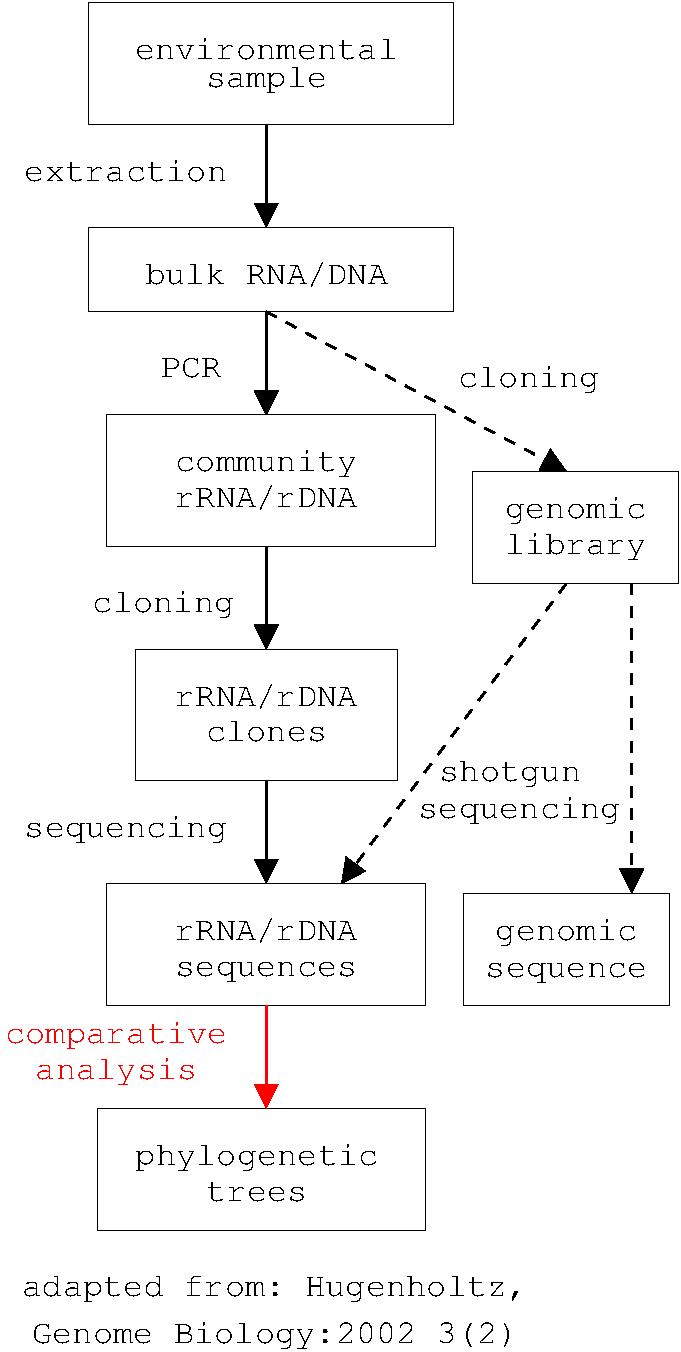
\includegraphics[height=5.5in]{figs/environmental}
\vspace{1in}
\end{minipage}
\end{slide}

%%%%%%%%%%%%%%%%%%%%%%%%%%%%%%%%%%%%%%%%%%%%%%%%%%%%%%%%%%%%%%%%%%%%%%%%%%
\begin{slide}
\begin{center}
\textbf{SSU-ALIGN: structural alignment of SSU rRNAs using CMs}
\end{center}

\includegraphics[width=10in]{figs/seq2tree-2013-ssualign-released}

\vfill
\end{slide}
%%%%%%%%%%%%%%%%%%%%%%%%%%%%%%%%%%%%%%%%%%%%%%%%%%%%%%%%%%%%%%%%%%%%
\begin{slide}
\begin{center}
\small
\textbf{SSU-ALIGN: HMM-based classification followed by CM alignment}
\end{center}

\center{\includegraphics[width=7.5in]{figs/ssualign-schematic}}

\vfill
\end{slide}
%%%%%%%%%%%%%%%%%%%%%%%%%%%%%%%%%%%%%%%%%%%%%%%%%%%%%%%%%%%%%%%%%%%%%%%%%%
\begin{slide}
\begin{center}
\textbf{Limitations of SSU-ALIGN}
\end{center}

\small
\begin{itemize}
\item 
not designed for genome annotation (only 1 hit allowed per target
sequence)
\item 
only works with SSU rRNA 
\begin{itemize}
  \item only archaeal, bacterial, and eukaryotic (no mitochondria, chloroplast, or microsporidia)
\end{itemize}
\item 
relatively slow
\end{itemize}

\normalsize
\begin{center}
\textbf{Design goals of RNAVORE}
\end{center}

\small
\begin{itemize}
\item 
able to annotate genomes
\item 
find and align all types of rRNA (SSU, LSU, 5S, 5.8S)
\item 
accompanying publication
\end{itemize}

\vfill
%%%%%%%%%%%%%%%%%%%%%%%%%%%%%%%%%%%%%%%%%%%%%%%%%%%%%%%%%%%%%%%%%%%%%%%%%%
\begin{slide}
\begin{center}
\small
\textbf{SSU-ALIGN used HMMER2 technology making genome annotation too slow}
\end{center}

\center{\includegraphics[width=7in]{figs/ssualign-schematic}}

\vfill
\end{slide}
\end{slide}
%%%%%%%%%%%%%%%%%%%%%%%%%%%%%%%%%%%%%%%%%%%%%%%%%%%%%%%%%%%%%%%%%%%%%%%%%%
\begin{slide}
\begin{center}
\small
\textbf{SSU-ALIGN versus \emph{A. aeolicus} genome (1.6 Mb)}
\end{center}

\center{\includegraphics[width=5.2in]{figs/ssu-align-aaeo-ss-1}}
%\center{\includegraphics[width=5.2in]{figs/ssu-align-aaeo-ss-2}}
\center{\includegraphics[width=5.2in]{figs/ssu-align-aaeo-ss-3}}

\vfill
\end{slide}
%%%%%%%%%%%%%%%%%%%%%%%%%%%%%%%%%%%%%%%%%%%%%%%%%%%%%%%%%%%%%%%%%%%%%%%%%%
\begin{slide}
\begin{center}
\small
\textbf{Infernal 1.1's cmscan: \emph{A. aeolicus} genome versus archaeal and
bacterial SSU and LSU CMs}
\end{center}

%\begin{itemize}
%\item Infernal 1.1: run each CM against full target sequence database.

\center{\includegraphics[width=6in]{figs/cmscan-aaeo-ss-0}}
\center{\includegraphics[width=7.5in]{figs/cmscan-aaeo-ss-1}}
\center{\includegraphics[width=5in]{figs/cmscan-aaeo-ss-3}}

%\end{itemize}

\vfill
\end{slide}
%%%%%%%%%%%%%%%%%%%%%%%%%%%%%%%%%%%%%%%%%%%%%%%%%%%%%%%%%%%%%%%%%%%%%%%%%%
\begin{slide}
\begin{center}
\small
\textbf{Infernal 1.1's cmscan: \emph{A. aeolicus} genome versus archaeal and
bacterial SSU and LSU CMs}
\end{center}

\center{\includegraphics[width=7.5in]{figs/cmscan-aaeo-ss-2}}

\vfill
\end{slide}
%%%%%%%%%%%%%%%%%%%%%%%%%%%%%%%%%%%%%%%%%%%%%%%%%%%%%%%%%%%%%%%%%%%%%%%%%%
\begin{slide}
\begin{center}
\small
\textbf{RNAVORE uses HMMER3/Infernal 1.1 to make genome annotation practical}
\end{center}

\begin{itemize}
\item Stage 1: all profile HMMs are run against all target
  sequences (\texttt{cmscan}): 
\begin{itemize}
\item F1:  SSV filter (local)
%\item F1B: Bias filter
\item F2: Viterbi filter (local)
%\item F2B: Bias filter
\item F3: Forward filter (local)
%\item F3B: Bias filter
\item Tabular output lists windows that survive Forward (SSV hits plus
  enough padding that we include full hit)
\end{itemize}
%\item Stage 2: Classify each target sequence based on best scoring
%  model from stage 1 (archaeal, bacterial, or eukaryotic?) and extract
%  hits to new fasta files.
%\item Stage 3: Pass model-specific subsequence files to corresponding
%  CMs to further refine boundaries and create alignments
%  (\texttt{cmsearch}).
\end{itemize}

\vfill
\end{slide}
%%%%%%%%%%%%%%%%%%%%%%%%%%%%%%%%%%%%%%%%%%%%%%%%%%%%%%%%%%%%%%%%%%%%%%%%%%
\begin{slide}
\begin{center}
\small
\textbf{Tabular output with \texttt{--trmF3} option}
\end{center}

\center{\includegraphics[width=10in]{figs/rnavore-aaeo-f3tbl-ss-1}}

\vfill
\end{slide}
%%%%%%%%%%%%%%%%%%%%%%%%%%%%%%%%%%%%%%%%%%%%%%%%%%%%%%%%%%%%%%%%%%%%%%%%%%
\begin{slide}
\begin{center}
\small
\textbf{RNAVORE uses HMMER3/Infernal 1.1 to make genome annotation practical}
\end{center}

\begin{itemize}
\item Stage 2: Classify each target sequence based on best scoring
  model from stage 1 (archaeal, bacterial, or eukaryotic?) and extract
  subsequences to new fasta files.
\item Stage 3: Pass model-specific subsequence files to corresponding
  CMs to refine boundaries and create alignments
  (\texttt{cmsearch}).
\end{itemize}

\vfill
\end{slide}
%%%%%%%%%%%%%%%%%%%%%%%%%%%%%%%%%%%%%%%%%%%%%%%%%%%%%%%%%%%%%%%%%%%%%%%%%%
\begin{slide}
\begin{center}
\small
\textbf{RNAVORE against \emph{A. aeolicus} genome}
\end{center}

\center{\includegraphics[width=6.5in]{figs/rnavore-aaeo-ss-1}}

\vfill
\end{slide}
%%%%%%%%%%%%%%%%%%%%%%%%%%%%%%%%%%%%%%%%%%%%%%%%%%%%%%%%%%%%%%%%%%%%%%%%%%
\begin{slide}
\begin{center}
\small
\textbf{RNAVORE does not report overlapping hits}
\end{center}

\center{\includegraphics[width=10in]{figs/rnavore-aaeo-tbl-ss-1}}

\vfill
\end{slide}
%%%%%%%%%%%%%%%%%%%%%%%%%%%%%%%%%%%%%%%%%%%%%%%%%%%%%%%%%%%%%%%%%%%%%%%%%%
%\begin{center}
%\textbf{RNAVORE development progress}
%\end{center}
%
%\begin{itemize}
%\item Initial aim was to change as little as possible, due to time constraints.
%
%\item Quickly realized I couldn't restrain myself from a massive
%  overhaul.
%
%\item \texttt{rvr-align} replaces \texttt{ssu-align} and is nearly a
%  compete re-write.
%\end{itemize}
%
%\vfill
%\end{slide}
%%%%%%%%%%%%%%%%%%%%%%%%%%%%%%%%%%%%%%%%%%%%%%%%%%%%%%%%%%%%%%%%%%%%%%%%%%
\begin{slide}
\begin{center}
\small
\textbf{A further wrinkle related to Infernal 1.1's truncated hit
  detection feature}
\end{center}

\small
\begin{itemize}
\item Infernal 1.1's \texttt{cmsearch} takes special care to identify
  truncated RNAs at \emph{beginning} and \emph{end} of sequences using specialized
  algorithms (Kolbe, Eddy, 2009).
%\item Each sequence goes through multiple ``passes'': 
%  \begin {itemize}
%  \item pass 1: looking for non-truncated hits (full sequence)
%  \item pass 2: allowing 5' truncations (W 5' most nucleotides)
%  \item pass 3: allowing 3' truncations (W 3' most nucleotides)
%  \item pass 4: allowing 5' and 3' truncations (only for seqs of
%    length $<=$ W)
%  \end{itemize}
%\item Since RNAVORE sequences are already subsequences, we have to be
%  careful:
%  \begin{itemize}
%  \item only windows that comprise entire sequence can go through all
%    passes
%  \item windows that include 5' terminus can go through passes 1 and 2 only
%  \item windows that include 3' terminus can go through passes 1 and 3 only
%  \item windows without either termini can go through pass 1 only
%  \end{itemize}
%\item for SSU libraries, most/all windows will comprise full sequence:
%  \begin{itemize}
%  \item each pass requires about 1 second
%  \item to save time, we do each pass only through all HMM stages,
%    and execute final (slow) CM stages only on the single best-scoring pass.
%  \end{itemize}
\end{itemize}

\vfill
\end{slide}
%%%%%%%%%%%%%%%%%%%%%%%%%%%%%%%%%%%%%%%%%%%%%%%%%%%%%%%%%%%%%%%%%%%%%%%%%%
\begin{slide}
\begin{center}
\small
\textbf{A further wrinkle related to Infernal 1.1's truncated hit
  detection feature}
\end{center}

\small
\begin{itemize}
\item Infernal 1.1's \texttt{cmsearch} takes special care to identify
  truncated RNAs at \emph{beginning} and \emph{end} of sequences using specialized
  algorithms (Kolbe, Eddy, 2009).
\item Each sequence goes through multiple ``passes'': 
  \begin {itemize}
  \item pass 1: looking for non-truncated hits (full sequence)
  \item pass 2: allowing 5' truncations (W 5' most nucleotides)
  \item pass 3: allowing 3' truncations (W 3' most nucleotides)
  \item pass 4: allowing 5' and 3' truncations (only for seqs of
    length $<=$ W)
  \end{itemize}
%\item Since RNAVORE sequences are already subsequences, we have to be
%  careful:
%  \begin{itemize}
%  \item only windows that comprise entire sequence can go through all
%    passes
%  \item windows that include 5' terminus can go through passes 1 and 2 only
%  \item windows that include 3' terminus can go through passes 1 and 3 only
%  \item windows without either termini can go through pass 1 only
%  \end{itemize}
%\item for SSU libraries, most/all windows will comprise full sequence:
%  \begin{itemize}
%  \item each pass requires about 1 second
%  \item to save time, we do each pass only through all HMM stages,
%    and execute final (slow) CM stages only on the single best-scoring pass.
%  \end{itemize}
\end{itemize}

\vfill
\end{slide}
%%%%%%%%%%%%%%%%%%%%%%%%%%%%%%%%%%%%%%%%%%%%%%%%%%%%%%%%%%%%%%%%%%%%%%%%%%
\begin{slide}
\begin{center}
\small
\textbf{A further wrinkle related to Infernal 1.1's truncated hit
  detection feature}
\end{center}

\small
\begin{itemize}
\item Infernal 1.1's \texttt{cmsearch} takes special care to identify
  truncated RNAs at \emph{beginning} and \emph{end} of sequences using specialized
  algorithms (Kolbe, Eddy, 2009).
\item Each sequence goes through multiple ``passes'': 
  \begin {itemize}
  \item pass 1: looking for non-truncated hits (full sequence)
  \item pass 2: allowing 5' truncations (W 5' most nucleotides)
  \item pass 3: allowing 3' truncations (W 3' most nucleotides)
  \item pass 4: allowing 5' and 3' truncations (only for seqs of
    length $<=$ W)
  \end{itemize}
\item Since RNAVORE sequences are already subsequences, we have to be
  careful:
  \begin{itemize}
  \item only windows that comprise entire sequence can go through all
    passes
  \item windows that include 5' terminus can go through passes 1 and 2 only
  \item windows that include 3' terminus can go through passes 1 and 3 only
  \item windows without either termini can go through pass 1 only
  \end{itemize}
%\item for SSU libraries, most/all windows will comprise full sequence:
%  \begin{itemize}
%  \item each pass requires about 1 second
%  \item to save time, we do each pass only through all HMM stages,
%    and execute final (slow) CM stages only on the single best-scoring pass.
%  \end{itemize}
\end{itemize}

\vfill
\end{slide}
%%%%%%%%%%%%%%%%%%%%%%%%%%%%%%%%%%%%%%%%%%%%%%%%%%%%%%%%%%%%%%%%%%%%%%%%%%
\begin{slide}
\begin{center}
\small
\textbf{A further wrinkle related to Infernal 1.1's truncated hit
  detection feature}
\end{center}

\small
\begin{itemize}
\item Infernal 1.1's \texttt{cmsearch} takes special care to identify
  truncated RNAs at \emph{beginning} and \emph{end} of sequences using specialized
  algorithms (Kolbe, Eddy, 2009).
\item Each sequence goes through multiple ``passes'': 
  \begin {itemize}
  \item pass 1: looking for non-truncated hits (full sequence)
  \item pass 2: allowing 5' truncations (W 5' most nucleotides)
  \item pass 3: allowing 3' truncations (W 3' most nucleotides)
  \item pass 4: allowing 5' and 3' truncations (only for seqs of
    length $<=$ W)
  \end{itemize}
\item Since RNAVORE sequences are already subsequences, we have to be
  careful:
  \begin{itemize}
  \item only windows that comprise entire sequence can go through all
    passes
  \item windows that include 5' terminus can go through passes 1 and 2 only
  \item windows that include 3' terminus can go through passes 1 and 3 only
  \item windows without either termini can go through pass 1 only
  \end{itemize}
\item for SSU libraries, most/all windows will comprise full sequence:
  \begin{itemize}
  \item each pass requires about 1 second
  \item to save time, we do each pass only through all HMM stages,
    and execute final (slow) CM stages only on the single best-scoring pass.
  \end{itemize}
\end{itemize}

\vfill
\end{slide}
%%%%%%%%%%%%%%%%%%%%%%%%%%%%%%%%%%%%%%%%%%%%%%%%%%%%%%%%%%%%%%%%%%%%%%%%%%
\begin{slide}
\begin{center}
\small
\textbf{RNAVORE development: still to do}
\end{center}

\small
\begin{itemize}
\item relax 10 Mb length requirement for \texttt{cmscan}
\item Add 5S, 5.8S, and other LSU/SSU (mitochondria, chloroplast)
\item Update \texttt{ssu-draw}, \texttt{ssu-mask}, \texttt{ssu-build}
  (maybe \texttt{ssu-prep} and \texttt{ssu-merge})
\item Add 'pin' search for faster SSU/LSU identification
\item Implement method for distinguishing chloroplast/cyanobacteria
  SSU and LSU
\item Write documentation and testsuite
\item Publish
\end{itemize}

\vfill
\end{slide}
%%%%%%%%%%%%%%%%%%%%%%%%%%%%%%%%%%%%%%%%%%%%%%%%%%%%%%%%%%%%%%%%%%%%%%%%%%
\begin{slide}
\begin{center}
\small
\textbf{Group I catalytic Introns}
\end{center}
%
\small
\begin{itemize}
\item self splicing ribozymes found in lower eukaryotes, higher
  plants, bacteria and bacteriophages
\item core secondary structure (modeled by Rfam) consists of 9 paired
  regions
\item often have ORFs inserted in loop regions
\item Genes they are found in:
\begin {itemize}
\item bacteria and mitochondria and chloroplast of lower euks: rRNA, mRNA, and tRNAs
\item nuclear lower euk genomes: only rRNA
\item higher plants mitochondria and chloroplast: a few tRNA and mRNA genes
\item Gram positive bacteriophages: widely distributed
\item Gram negative bacteriophages: T4, T-even and T7-like
\end{itemize}
\end{itemize}

\vfill
\end{slide}
%%%%%%%%%%%%%%%%%%%%%%%%%%%%%%%%%%%%%%%%%%%%%%%%%%%%%%%%%%%%%%%%%%%%%%%%%%
\begin{slide}
\begin{center}
\small
\textbf{Rfam NAR paper Table 1: Rfam 12.0 versus Rfam 11.0 for 200 families}
\end{center}

\center{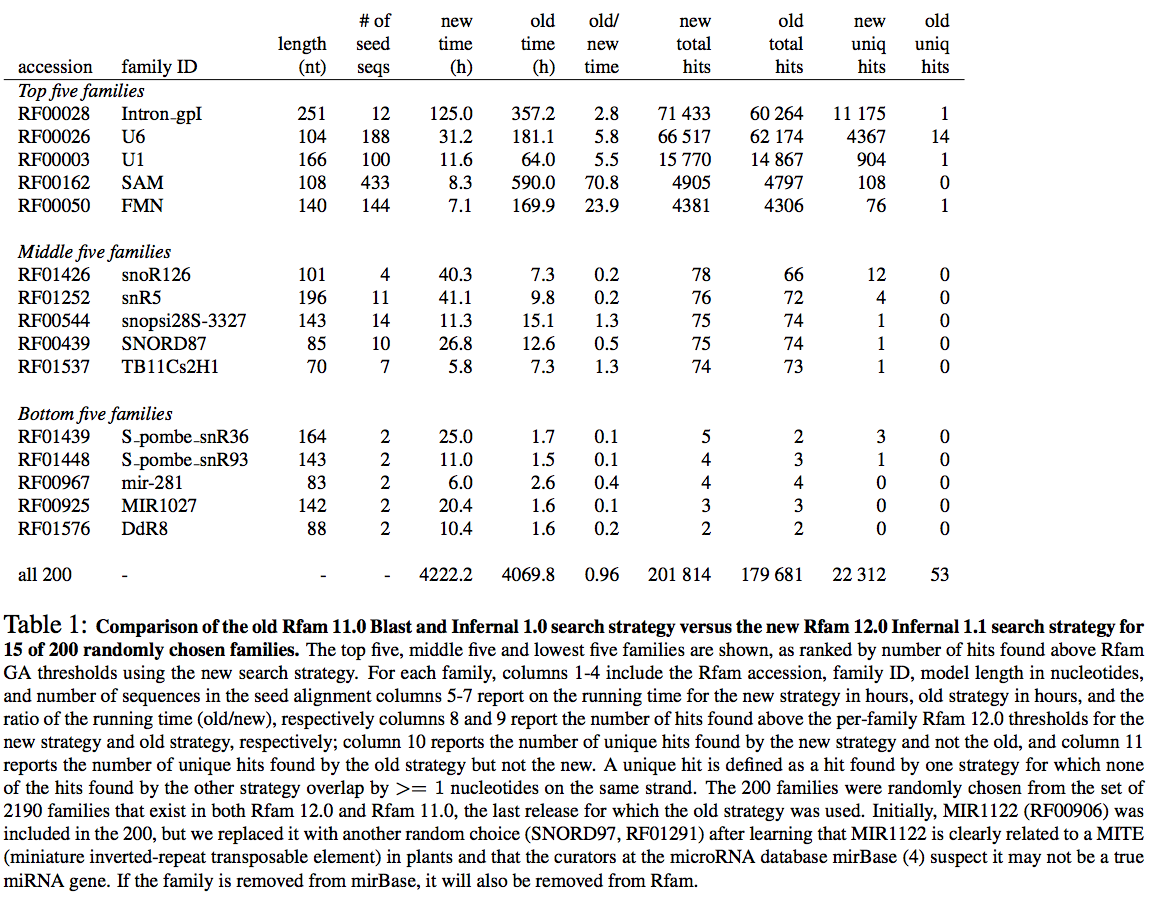
\includegraphics[width=8.5in]{figs/rfam-nar-table1-preprint-ss}}

\vfill
\end{slide}
%%%%%%%%%%%%%%%%%%%%%%%%%%%%%%%%%%%%%%%%%%%%%%%%%%%%%%%%%%%%%%%%%%%%%%%%%%
\begin{slide}
\center{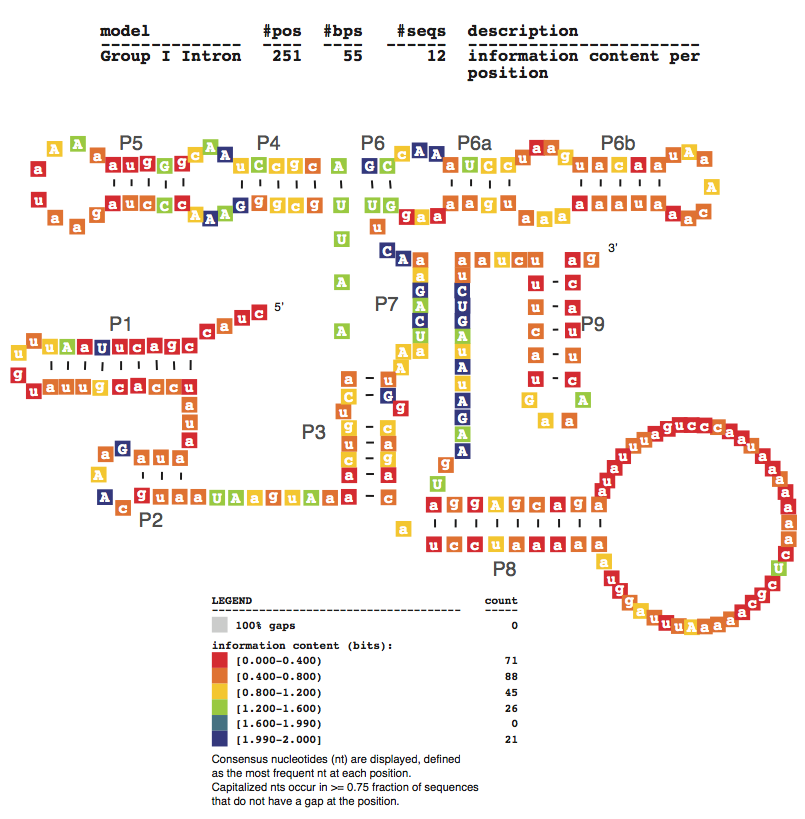
\includegraphics[height=8in]{figs/RF00028-ss-info-ss-1}}
\vfill
\end{slide}
%%%%%%%%%%%%%%%%%%%%%%%%%%%%%%%%%%%%%%%%%%%%%%%%%%%%%%%%%%%%%%%%%%%%%%%%%%
\begin{slide}
\center{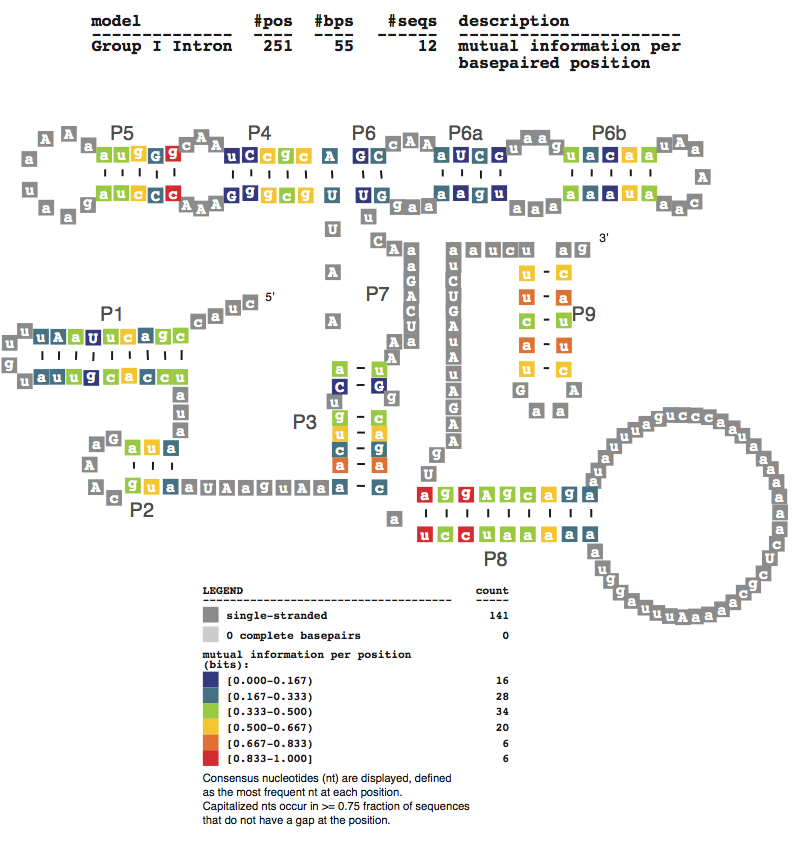
\includegraphics[height=8in]{figs/RF00028-ss-mutinfo-ss-1}}
\vfill
\end{slide}
%%%%%%%%%%%%%%%%%%%%%%%%%%%%%%%%%%%%%%%%%%%%%%%%%%%%%%%%%%%%%%%%%%%%%%%%%%
\begin{slide}
\center{\includegraphics[height=8in]{figs/RF00028-ss-ifreq-ss-1}}
\vfill
\end{slide}
%%%%%%%%%%%%%%%%%%%%%%%%%%%%%%%%%%%%%%%%%%%%%%%%%%%%%%%%%%%%%%%%%%%%%%%%%%
\begin{slide}
\center{\includegraphics[height=8in]{figs/RF00028-ss-ilen-ss-1}}
\vfill
\end{slide}
%%%%%%%%%%%%%%%%%%%%%%%%%%%%%%%%%%%%%%%%%%%%%%%%%%%%%%%%%%%%%%%%%%%%%%%%%%
\begin{slide}
\center{\includegraphics[height=8in]{figs/RF00028-ss-dall-ss-1}}
\vfill
\end{slide}
%%%%%%%%%%%%%%%%%%%%%%%%%%%%%%%%%%%%%%%%%%%%%%%%%%%%%%%%%%%%%%%%%%%%%%%%%%
\begin{slide}
\small
\center{\includegraphics[height=8.5in]{figs/euk-phylogeny-RF00028-counts-110314-1}}
\vfill
\end{slide}
%%%%%%%%%%%%%%%%%%%%%%%%%%%%%%%%%%%%%%%%%%%%%%%%%%%%%%%%%%%%%%%%%%%%%%%%%%
\begin{slide}
\begin{center}
\small
\textbf{GISSD: Group I Intron Sequence and Structure Database}
\end{center}

\center{
\includegraphics[width=10in]{figs/gissd-banner}}

\center{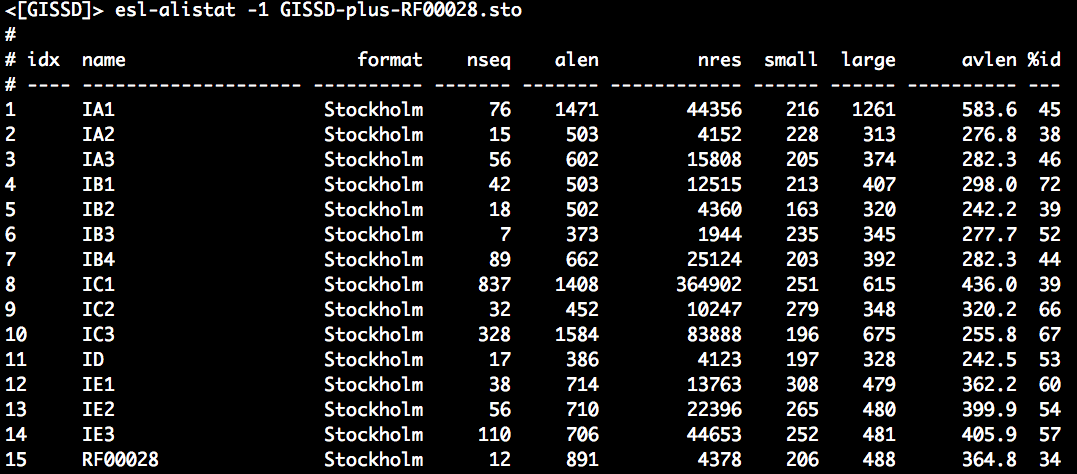
\includegraphics[width=10in]{figs/gissd-alistat-ss-1}}

\vfill
\end{slide}
%%%%%%%%%%%%%%%%%%%%%%%%%%%%%%%%%%%%%%%%%%%%%%%%%%%%%%%%%%%%%%%%%%%%%%%%%%
\begin{slide}
\begin{center}
\small
\textbf{GISSD CM statistics}
\end{center}

\center{\includegraphics[width=10in]{figs/gissd-cmstat-ss-1}}

\vfill
\end{slide}
%%%%%%%%%%%%%%%%%%%%%%%%%%%%%%%%%%%%%%%%%%%%%%%%%%%%%%%%%%%%%%%%%%%%%%%%%%
\begin{slide}
\begin{center}
\small
\textbf{Measuring specificity of GISSD models against training
  sequences using RNAVORE} 
\end{center}
%\center{\includegraphics[width=10in]{figs/gissd-specificity-ss-1-PRESENTED-INCORRECT}}
\center{\includegraphics[width=10in]{figs/gissd-specificity-ss-1}}
\vfill
\end{slide}
%%%%%%%%%%%%%%%%%%%%%%%%%%%%%%%%%%%%%%%%%%%%%%%%%%%%%%%%%%%%%%%%%%%%%%%%%%
\begin{slide}
\begin{center}
\small
\textbf{Searching Rfamseq with GISSD models}
\end{center}

\small
\begin{center}
\begin{tabular}{l|r|rrr|r}
\tt
        & \# RF00028 & \# hits   & \# hits& \# hits& total     \\
type    & seed seqs  & total     & common & unique & CPU hours \\ \hline
IA1     & 3          & ?         & ?      & ?      & ? \\
IA2     & 1          &  1722     & 823    & 899    & 50 \\
IA3     &            &   958     & 401    & 557    & 14 \\
IB1     &            &  3949     & 1033   & 2916   & 32 \\
IB2     &            & 1861     & 467    & 1394   & 31 \\
IB3     &            & 479     & 136    & 343    & 40 \\
IB4     &  1         & 5717     & 2400   & 3317   & 39 \\
IC1     &  3         & 8475     & 5385   & 3090   & 24 \\
IC2     &            & 4870     & 3858   & 1012   & 22 \\
IC3     & 4          & 72692     & 66033  & 6659   & 136 \\
ID      &            & 572     & 0      & 572    & 29 \\
IE1     &            & 1305     & 10     & 1295   & 12 \\
IE2     &            & 1377     & 8      & 1369   & 12 \\
IE3     &            & 1379     & 1      & 1378   & 13 \\
        &            &          &        &        &    \\
total   & 12         & 105356*   & 80555* & 24801  & 454 \\
        &           &           &        &    \\
RF00028 & -         & 71421     & 71421  & -      & 125 \\
\end{tabular}

\begin{description}
\item[*] contains overlaps
\end{description}

\end{center}

\vfill
\end{slide}
%%%%%%%%%%%%%%%%%%%%%%%%%%%%%%%%%%%%%%%%%%%%%%%%%%%%%%%%%%%%%%%%%%%%%%%%%
\end{document}

